\begin{figure}
%\makebox[\textwidth]{\framebox[10cm]{\rule{0pt}{250pt}}}  
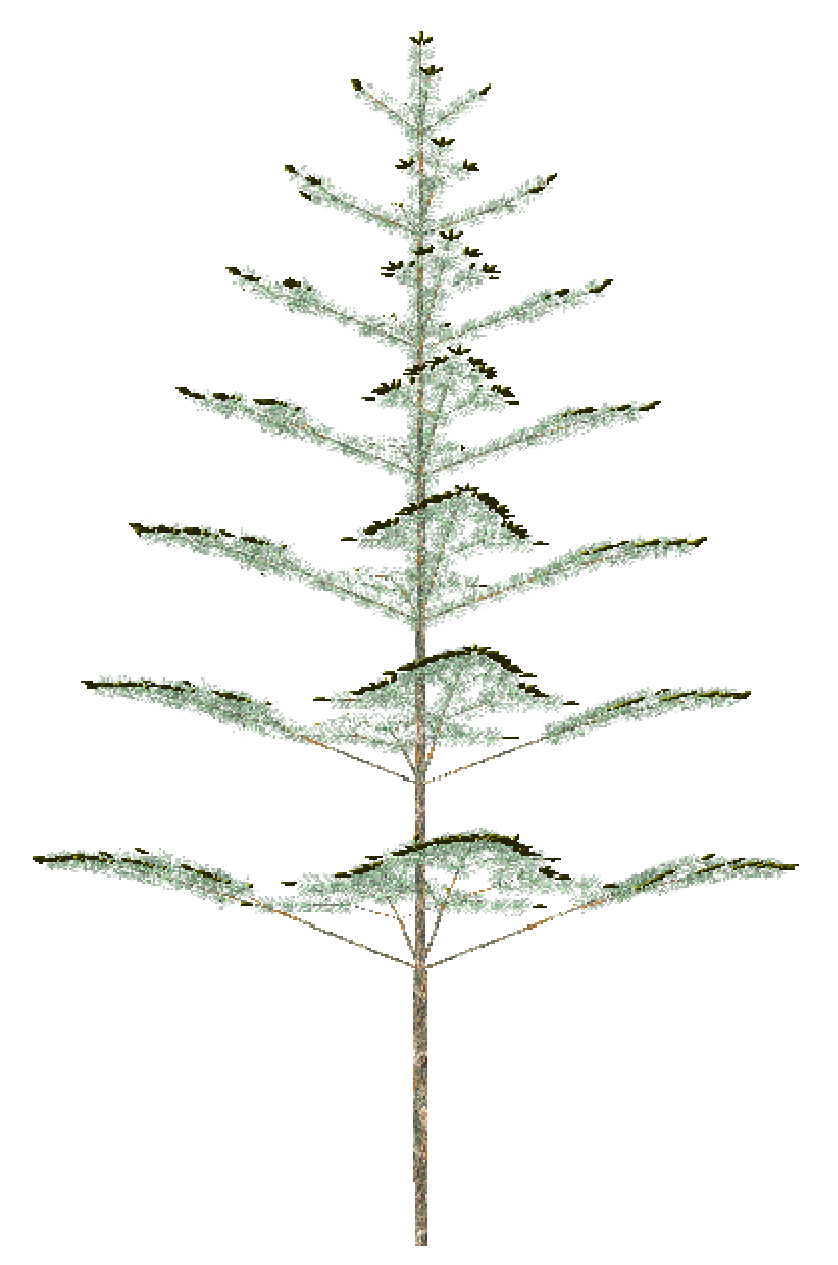
\includegraphics[scale=0.25]{pineL8}
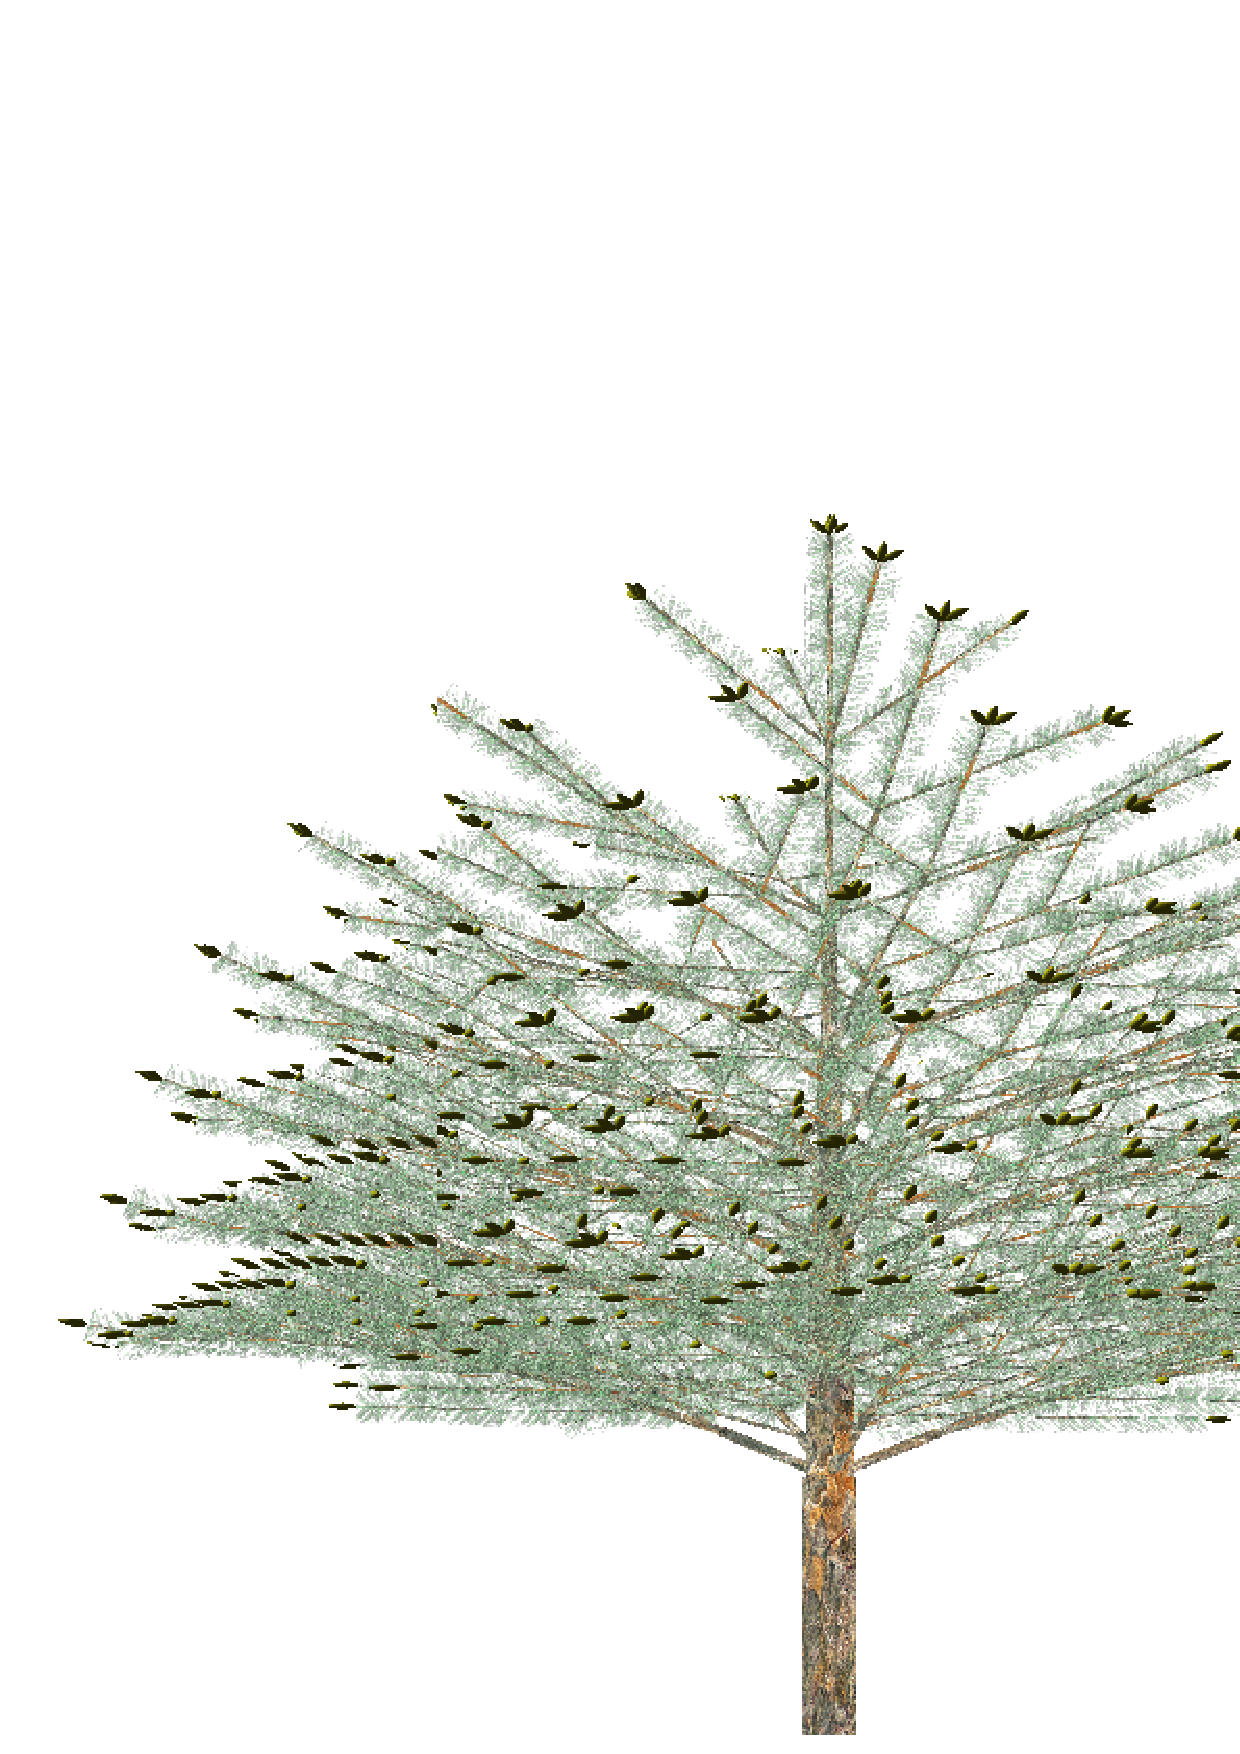
\includegraphics[scale=0.20]{pine8FEM98}
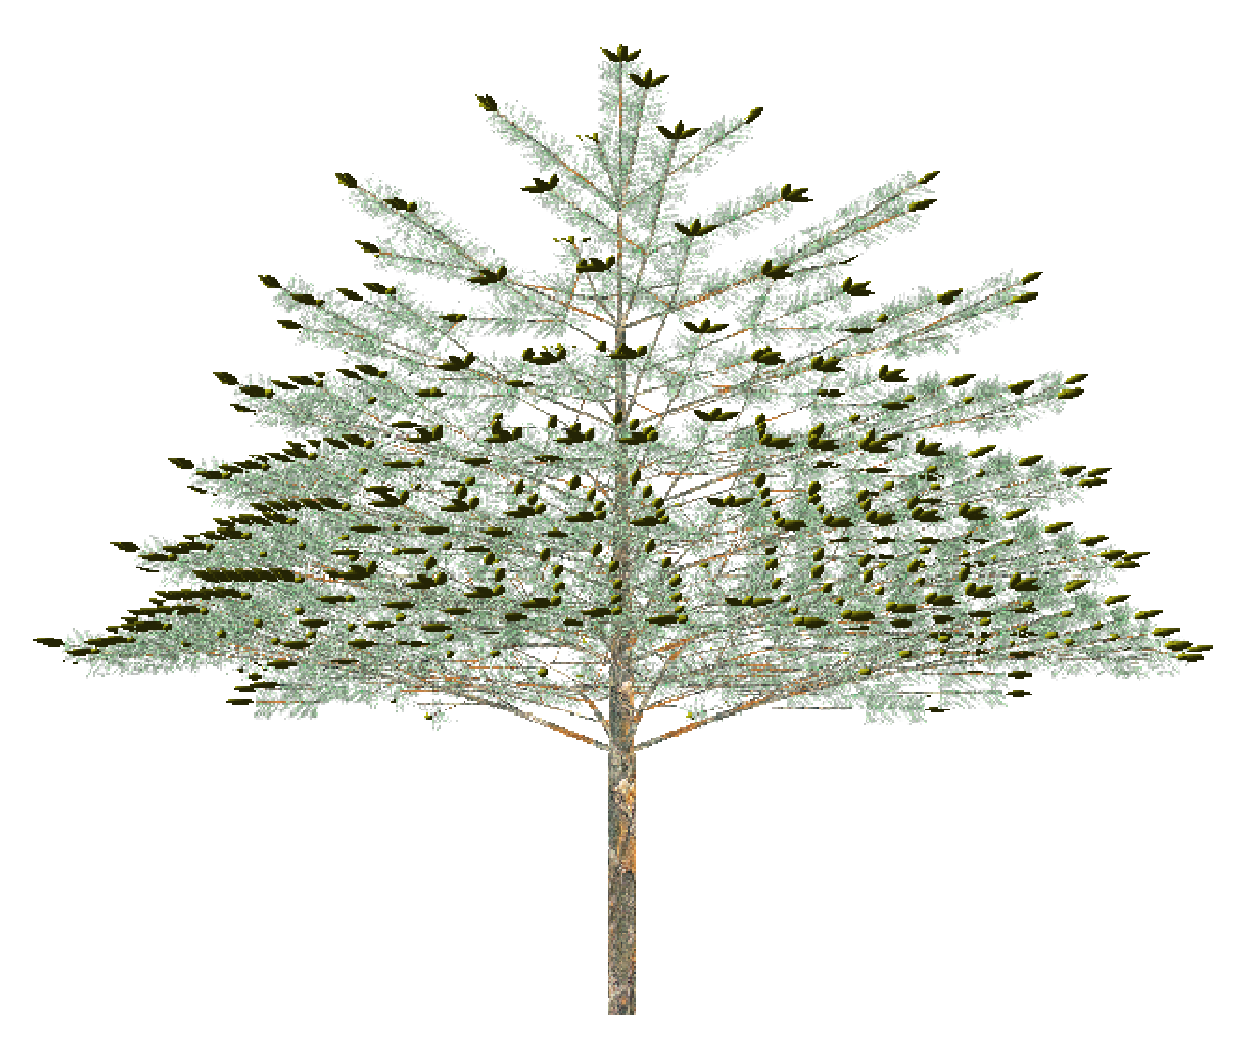
\includegraphics[scale=0.20]{pine8F1}   
\caption{The development of three  pines after eight development steps
when architectural  development is according to L  program of Appendix
\ref{sec:L1} and  metabolic functioning is  as in \citet{perttunen:96,
perttunen:98}. We  omit some functions  of LIGNUM, e.g. the  number of
secondary buds  as a function foliage  mass of mother  segment and let
the L-system determine  branching.  Leftmost: Development according to
L program only, middle and right: interaction of L language and LIGNUM
depicting the effect of  foliage mortality.  Middle: Foliage remains 5
years.  Length  = 3.5  m, diameter  at base =  10 cm.   Right: Foliage
remains 1 year.  Length = 2.7 m, diameter at base 6 cm.}
\label{fig:pine}
\end{figure}

